%!Mode::"UTF-8"
\documentclass[12pt]{article}

% 页面设置
\usepackage{geometry}
\geometry{left=2.5cm, right=2.5cm, top=2.5cm, bottom=2.5cm}
\usepackage{graphicx}
\usepackage{ctex}
\usepackage{fontspec}
\usepackage{setspace}

%高亮使用的颜色
\usepackage{xcolor}  	
\definecolor{commentcolor}{RGB}{0,121,121}
\definecolor{stringcolor}{RGB}{190,49,49}
\definecolor{keywordcolor}{RGB}{0,128,0}

% 代码设置
\usepackage{listings}
\usepackage{color}
\setmonofont{Consolas}
\definecolor{listing}{gray}{0.97}
\lstset{
	backgroundcolor=\color{listing},
	basicstyle=\footnotesize,
	commentstyle=\color{commentcolor},	%注释颜色
	keywordstyle=\color{keywordcolor}\textbf,	%关键词颜色
	stringstyle=\color{stringcolor},
	numbers=left,
	numberstyle=\footnotesize,
	stepnumber=1,
	aboveskip={0.5\baselineskip},
	belowskip={0.5\baselineskip},
	columns=fullflexible,
	breaklines=true,
	breakatwhitespace=true,
	frame=single,
	basicstyle=\ttfamily,
	numberstyle=\ttfamily,
	tabsize=3
}

% 字体设置
\setmainfont{Times New Roman}
\setCJKmainfont{SimSun}
\setCJKsansfont{SimHei}
\usepackage[version=4]{mhchem}
\usepackage{mathtools}
\usepackage{diffcoeff}

% 表格设置
\usepackage{makecell}
\newcommand{\addcell}[2][4]{\makecell{\zihao{#1}\textsf{#2}}}
\usepackage{titlesec}
\usepackage{booktabs}
\usepackage{tabularx}

% 设置图注、表注
\usepackage{caption}
\usepackage{bicaption}
\captionsetup{labelsep=quad, font={small, bf}, skip=2pt}
\DeclareCaptionOption{english}[]{
    \renewcommand\figurename{Fig.}
    \renewcommand\tablename{Table}
}
\captionsetup[bi-second]{english}

% 设置页眉
\usepackage{fancyhdr}
\pagestyle{fancy}
\fancypagestyle{preContent}{
    \fancyhead[L]{\zihao{-5} 机器学习基础}
    \fancyhead[C]{\zihao{-5} 作业6\ \ 决策树模型}
    \fancyhead[R]{\zihao{-5} 1800011828\ 王宇哲}
}
\pagestyle{preContent}

%	设置首页页眉页脚
\fancypagestyle{plain}{
	\fancyhead[L]{\zihao{-5} 机器学习基础}
	\fancyhead[C]{\zihao{-5} 作业6\ \ 决策树模型}
	\fancyhead[R]{\zihao{-5} 1800011828\ 王宇哲}
	\cfoot{}
}

% 设置标题格式
\titleformat*{\section}{\zihao{4}\sffamily}
\titleformat*{\subsection}{\zihao{-4}\sffamily}
\titleformat*{\subsubsection}{\zihao{-4}\sffamily}
\titlespacing*{\section}{0pt}{10pt}{10pt}
\titlespacing*{\subsection}{0pt}{10pt}{5pt}
\titlespacing*{\subsubsection}{0pt}{10pt}{5pt}

% 设置引用格式
\usepackage[super,round,comma,compress]{natbib}

\usepackage{amsmath}
\usepackage{amssymb}

%设置封面
\begin{document}
    % 标题页
    \begin{titlepage}
    	% 页眉
    	\thispagestyle{plain}
        % 图片
        \begin{figure}[h]
            \centering
            \includegraphics[width=0.7\textwidth]{pku.png}
        \end{figure}
        \vspace{60pt}
        % 标题
        \centerline{\zihao{-0} \textsf{机器学习基础}}
        \vspace{20pt} % 空行
        \centerline{\zihao{-0} \textsf{课程上机试验报告}}
        \vspace{70pt} % 空行
        \begin{center}
            \begin{tabular}{cp{5.5 cm}}
                % 题目
                \addcell[2]{{\Huge 试验内容:\ }} & \addcell[2]{{\Huge 决策树模型}} \\
                \cline{2-2}
            \end{tabular}
        \end{center}
        \vspace{60pt} % 空行
        \begin{center}
            \doublespacing
            \begin{tabular}{cp{5cm}}
                % 姓名
                \addcell{姓\phantom{空格}名:\ } & \addcell{王宇哲} \\
                \cline{2-2}
                % 学号
                \addcell{学\phantom{空格}号:\ } & \addcell{1800011828}\\
                \cline{2-2}
            \end{tabular}
        \end{center}
       
    \end{titlepage}

\section{题目1}
	\subsection{实验题目}
	从UCI(http://archive.ics.uci.edu/ml/)上选择数据集对C4.5和CART算法生成的决策树进行实验比较。

               
      
\subsection{实验数据}
题目1使用的数据集为UCI上的wine数据集(https://archive.ics.uci.edu/ml/datasets/Wine),在scikit-learn库中也集成了该数据集。Wine数据集包含了种植在意大利相同地区的、被分为class\_0、class\_1、class\_2三类的178个红酒样本及其13维化学分析数据,适用于一般的分类问题。


\subsection{实验工具}
实验在个人LEVENO YOGA 710笔记本电脑上进行,主要硬件条件为:处理器Intel i5-7200U CPU,内存大小8.0 GB,显卡NVIDIA Geforce 940MX;操作系统为Windows 10 64位系统。\par 
实验使用语言为python,具体版本为python 3.7.0,通过Anaconda安装了Matplotlib、NumPy、pandas、scikit-learn等常用库。实验代码编写和运行均在Jupyter Notebook上进行,具体版本为Jupyter Notebook 6.3.0。



\subsection{实验方法}
实验采用的算法为经典的C4.5和CART决策树算法。经典C4.5、CART算法的原理在课程中已经进行详细讨论,此处不再赘述。\par
实验使用sklearn.tree库生成C4.5和CART决策树,通过调节tree.DecisionTreeClassifier函数的参数criterion='entropy'和criterion='gini'在C4.5和CART决策树之间切换。\par 
实验的具体操作方法如下。首先导入实验所需的必要的库,载入wine数据集的数据:
\begin{lstlisting}[language=python]
	from matplotlib import pyplot as plt
	import pandas as pd
	import numpy as np
	from sklearn import datasets, tree, model_selection, metrics
	
	from sklearn.datasets import load_wine
	data = load_wine()
	X = data.data
	Y = data.target
	df = pd.DataFrame(data.data, columns=data.feature_names)
	df['target'] = data.target
\end{lstlisting}
随后定义绘制决策树的函数tree\_draw和决策树训练函数tree\_train,绘制决策树时使用sklearn库集成的tree.plot\_tree模块进行绘图,训练决策树时将数据集按照9:1的比例随机划分成训练集和测试集,在测试集上检验所得决策树的泛化性能:
\begin{lstlisting}[language=python]
	def tree_draw(tree_type='CART', criterion='gini', figsize=(10,6)):
		dtree = tree.DecisionTreeClassifier(criterion=criterion)
		dtree.fit(X, Y)
	
		fn=['Alcohol','Malic acid','Ash', 'Alcalinity of ash', 'Magnesium', 'Total phenols', 'Flavanoids', 'Nonflavanoid phenols', 'Proanthocyanins', 'Color intensity', 'Hue', 'OD280/OD315 of diluted wines', 'Proline']
		cn=['class_0', 'class_1', 'class_2']
		fig, axes = plt.subplots(nrows = 1,ncols = 1,figsize = figsize, dpi=1000)
		tree.plot_tree(dtree, feature_names = fn, class_names=cn, filled = True, rounded = True);
		fig.savefig('tree_' + str(tree_type) + '.png')
	
	
	def tree_train(criterion='gini'):
		X_train, X_test, Y_train, Y_test = model_selection.train_test_split(df[data.feature_names], df['target'], test_size = 0.1)
		dtree = tree.DecisionTreeClassifier(criterion=criterion)
		dtree.fit(X_train, Y_train)
		Y_pred = dtree.predict(X_test)
		accuracy = metrics.accuracy_score(Y_test, Y_pred)
		return accuracy
\end{lstlisting}
随后分别训练C4.5和CART决策树,重复1000次,输出决策树预测准确率的平均值,并绘制在整个样本集上训练得到的C4.5和CART决策树的可视化图形:
\\
\begin{lstlisting}[language=python]
	for tree_type, criterion, figsize in [('CART', 'gini', (18,6)), ('C4.5', 'entropy', (10,6))]:
		accuracy_list = []
	
		for i in range(0, 1000):
			ac = tree_train(criterion=criterion)
			accuracy_list.append(ac)
	
		tree_draw(tree_type=tree_type, criterion=criterion, figsize=figsize)
	
		print('average accuracy of decision tree ' + '(' + str(tree_type) + '): ' + str("%.4f" % np.mean(accuracy_list)))
\end{lstlisting}


\subsection{实验结果}
实验代码总运行时长为$39.0\ \ {\rm s}$。训练得到的C4.5决策树如\textbf{图1}所示,C4.5算法生成的决策树在测试集上的平均准确率为0.9342。
\begin{figure}[h]
	\centering
	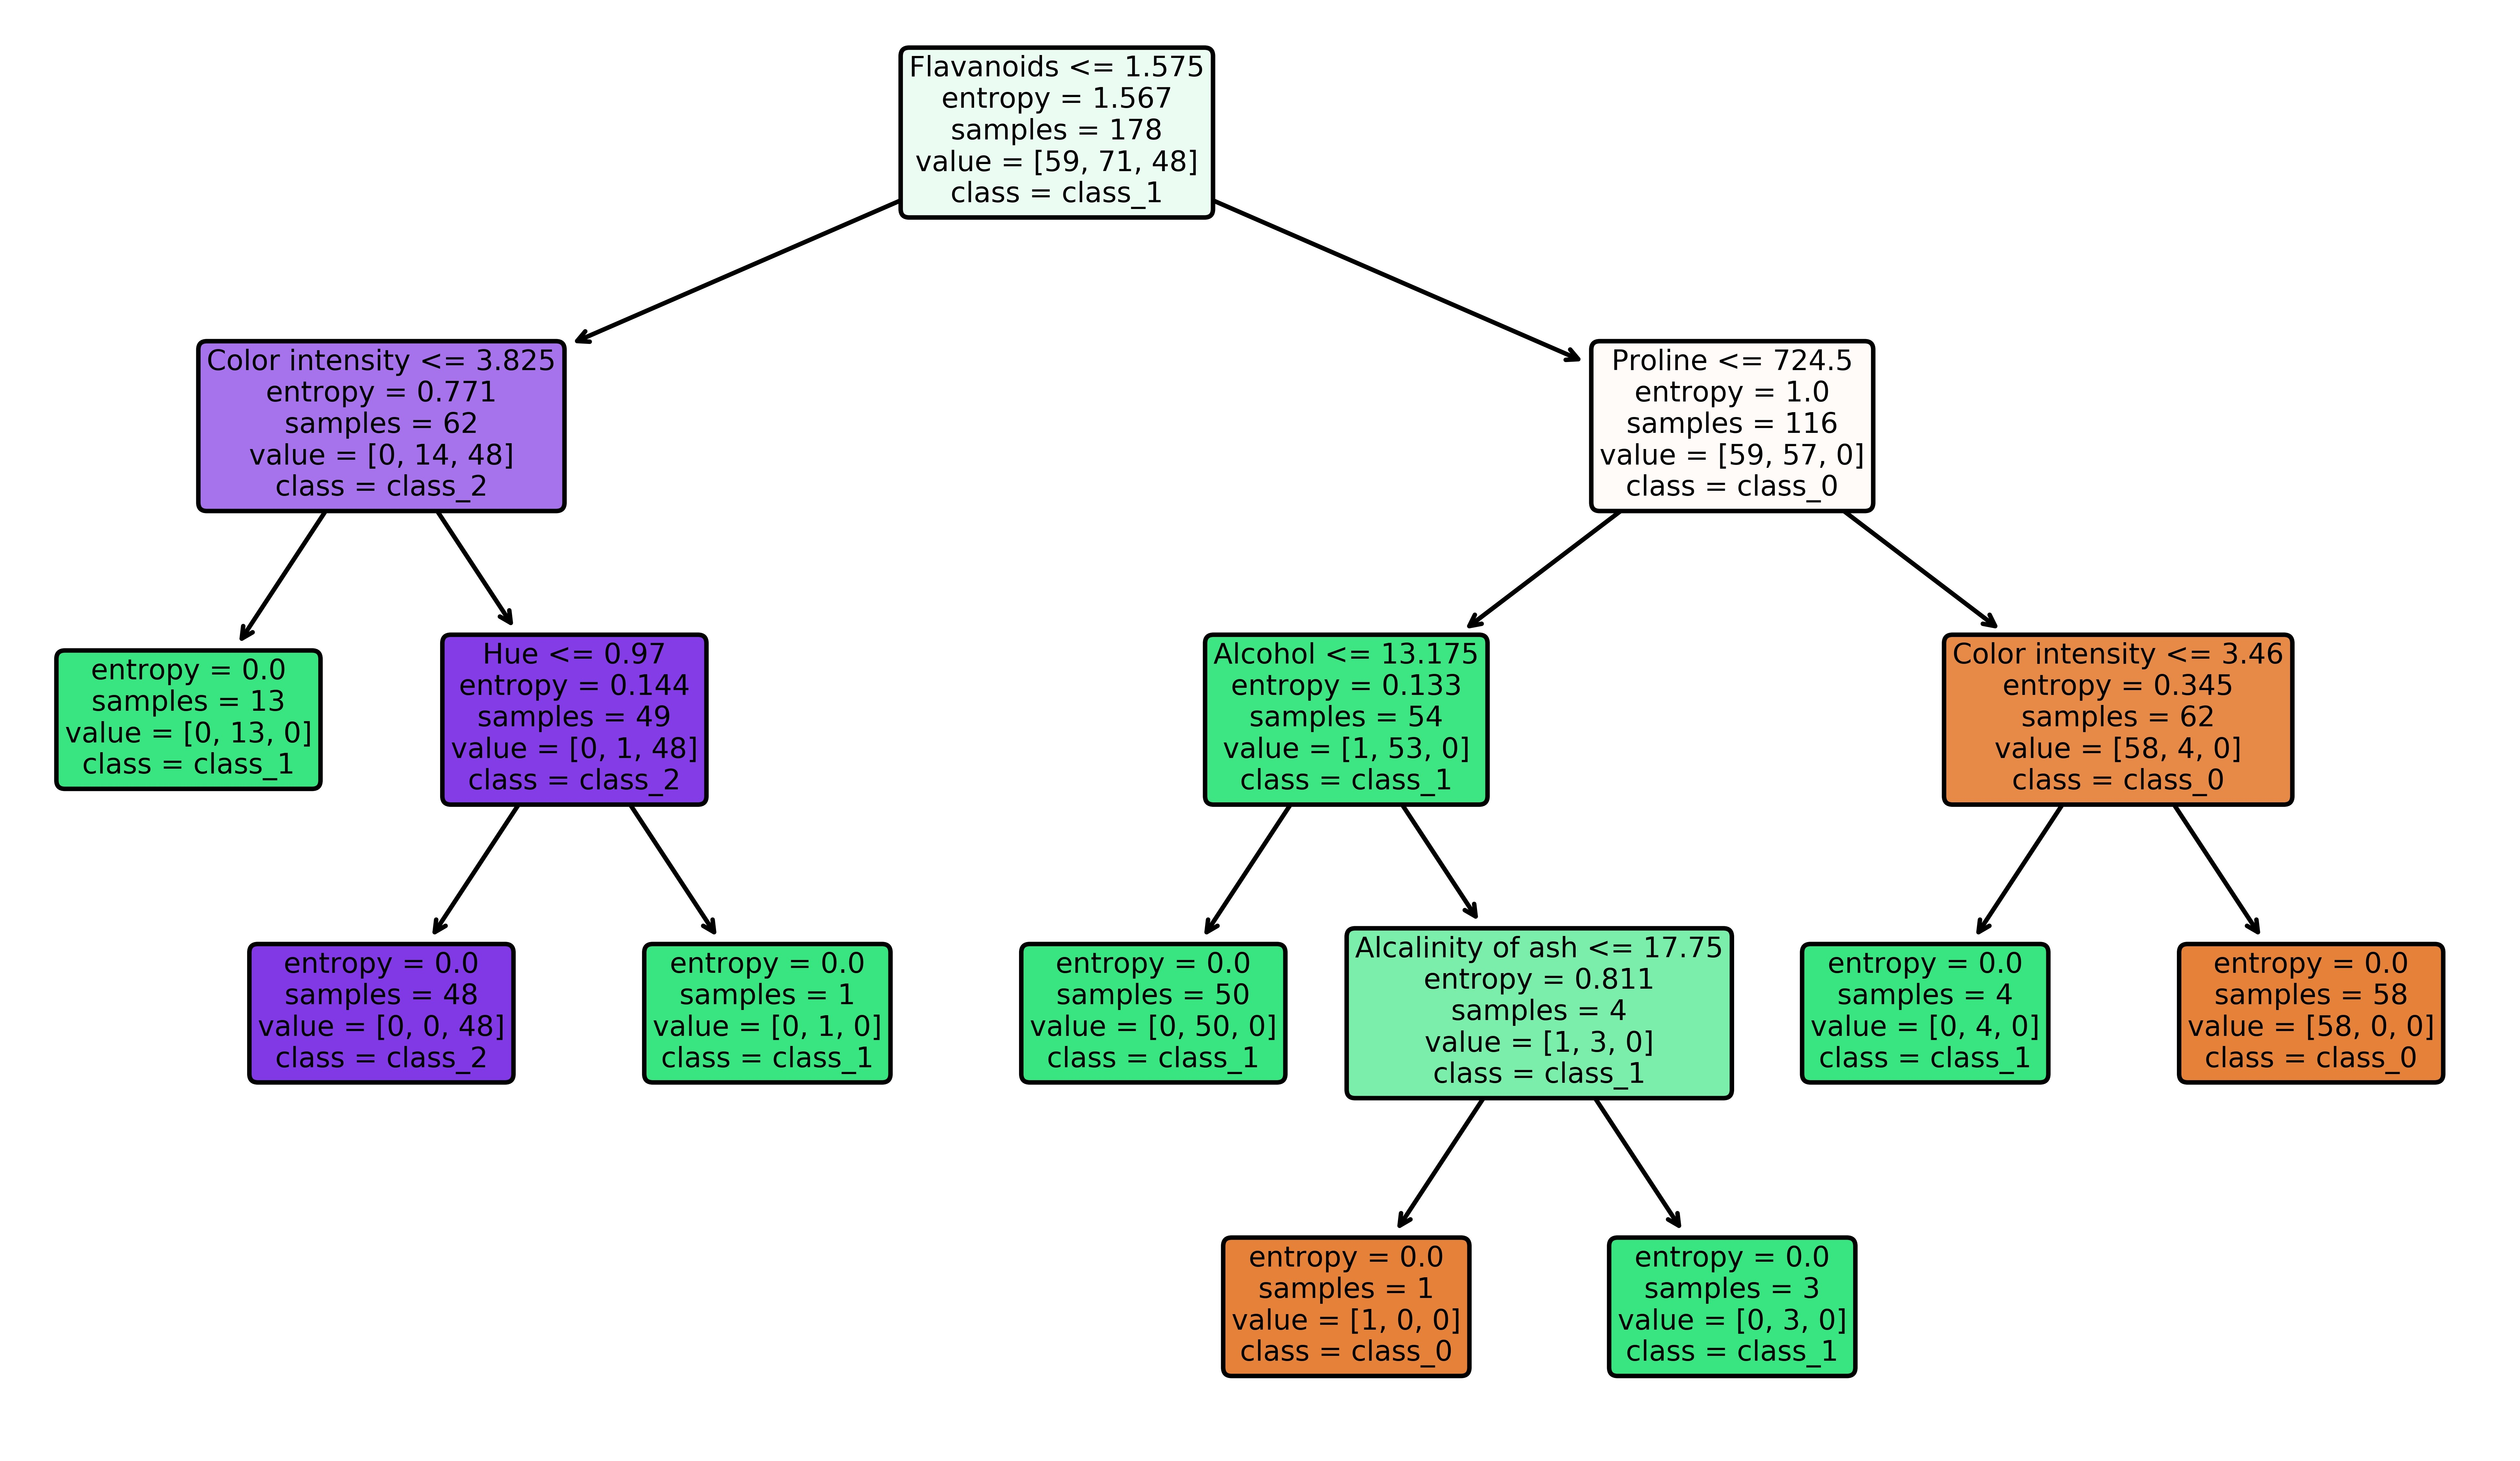
\includegraphics[width=0.9\textwidth]{tree_C45.jpg}
	\bicaption{C4.5决策树}{C4.5 Decision Tree}
\end{figure}
\par 

训练得到的CART决策树如\textbf{图2}所示,CART算法生成的决策树在测试集上的平均准确率为0.8989。

\begin{figure}[h]
	\centering
	\includegraphics[width=1\textwidth]{tree_CART.jpg}
	\bicaption{CART决策树}{CART Decision Tree}
\end{figure}
\par 


\vbox{}

\subsection{结果分析}
对比\textbf{图1}和\textbf{图2}可以发现,在wine数据集上,未剪枝的CART决策树相比C4.5决策树产生了更多的内部结点,CART算法比C4.5算法产生了更深的决策树。\par 
根据1.5的实验结果,可以分析认定:对于本题所用的wine数据集,C4.5算法产生的决策树在测试集上的准确率(0.9342)高于CART算法产生的决策树(0.8989),因此具有更优的表现。分析可知:CART算法产生的决策树在测试集上的准确率偏低,可能是由于未剪枝的CART决策树产生了一定的过拟合现象,导致在训练集上的泛化性能低于C4.5决策树。
\vbox{}

\newpage
\section{题目2}
\subsection{实验题目}
对C4.5算法设计一种新剪枝处理算法,并从UCI上选择数据集对新算法和已有算法进行实验比较。
\vbox{}
\subsection{实验数据}
同1.2,不再赘述。

\subsection{实验工具}
同1.3,不再赘述。
\vbox{}
\subsection{实验方法}
实验设计的剪枝处理算法参考了Breiman et al.提出的决策树CCP (Cost Complexity Pruning, 代价复杂度)剪枝算法\citealp{breiman}。具体地,CCP剪枝算法对代价复杂度函数 (cost-complexity function)进行优化:
$$
R_\alpha (T) = R(T) + \alpha \cdot | T |
$$
其中$R(T)$是叶结点总的训练误差,$|T|$是叶结点的数目,$\alpha$为复杂度参数。而对于某个特定结点$t$,满足
$$
R_\alpha (t) = R(t) + \alpha 
$$
对于以$t$为根结点的子树,有
$$R(T_{t})=\sum_{t\in L^{\prime}}R(t^{\prime})$$
其中$L$是子树$T_{t}$的叶结点的集合。子树$T_{t}$的代价复杂度为
$$
R_{\alpha}(T_{t})=R(T_{t})+\alpha|T_{t}|
$$
若满足
$$
R_{\alpha}(T_{t})=R_{\alpha}(t)
$$
则在结点$t$处的划分是无意义的。此时$\alpha$的值满足
$$
\alpha_{eff}(t)=\frac{R(t)-R(T_{t})}{|T|-1}
$$
对决策树的每个结点计算$\alpha$的值,在$\alpha$最小处进行剪枝。该过程重复进行,直至决策树仅保留根结点,在此过程中产生一系列$\alpha$值及其对应的决策树$T$。在训练集上分别测试各决策树的预测准确率,选择预测准确率最高的决策树作为最终生成的决策树,从而获得最优的泛化性能。\par 
该C4.5决策树CCP剪枝算法的代码实现示意如下:
\begin{lstlisting}[language=python]
	from matplotlib import pyplot as plt
	import pandas as pd
	import numpy as np
	from sklearn import datasets, tree, model_selection, metrics
	
	from sklearn.datasets import load_wine
	data = load_wine()
	X = data.data
	Y = data.target
	df = pd.DataFrame(data.data, columns=data.feature_names)
	df['target'] = data.target
	
	X_train, X_test, Y_train, Y_test = model_selection.train_test_split(df[data.feature_names], df['target'], test_size = 0.1)
	
	path=tree.DecisionTreeClassifier(criterion='entropy').\
	cost_complexity_pruning_path(X_train, Y_train)
	ccp_alphas, impurities = path.ccp_alphas, path.impurities
	
	fig, ax = plt.subplots(dpi=1000)
	ax.plot(ccp_alphas[:-1], impurities[:-1], marker='o', drawstyle="steps-post")
	ax.set_xlabel("effective alpha")
	ax.set_ylabel("total impurity of leaves")
	ax.set_title("Total Impurity vs effective alpha for training set")
	
	clfs = []
	for ccp_alpha in ccp_alphas:
		clf = tree.DecisionTreeClassifier(ccp_alpha=ccp_alpha)
		clf.fit(X_train, Y_train)
		clfs.append(clf)
	
	print("Number of nodes in the last tree is: {} with ccp_alpha: {} and a depth of: {}".format(
	clfs[-1].tree_.node_count, ccp_alphas[-1],clfs[-1].tree_.max_depth))
	
	clfs = clfs[:-1]
	ccp_alphas = ccp_alphas[:-1]
	
	node_counts = [clf.tree_.node_count for clf in clfs]
	depth = [clf.tree_.max_depth for clf in clfs]
	fig, ax = plt.subplots(2, 1, dpi=1000)
	ax[0].plot(ccp_alphas, node_counts, marker='o', drawstyle="steps-post")
	ax[0].set_xlabel("alpha")
	ax[0].set_ylabel("number of nodes")
	ax[0].set_title("Number of nodes vs alpha")
	ax[1].plot(ccp_alphas, depth, marker='o', drawstyle="steps-post")
	ax[1].set_xlabel("alpha")
	ax[1].set_ylabel("depth of tree")
	ax[1].set_title("Depth vs alpha")
	fig.tight_layout()
	
	train_scores = [clf.score(X_train, Y_train) for clf in clfs]
	test_scores = [clf.score(X_test, Y_test) for clf in clfs]
	fig, ax = plt.subplots(dpi=1000)
	ax.set_xlabel("alpha")
	ax.set_ylabel("accuracy")
	ax.set_title("Accuracy vs alpha for training and testing sets")
	ax.plot(ccp_alphas, train_scores, marker='o', label="train",
	drawstyle="steps-post")
	ax.plot(ccp_alphas, test_scores, marker='o', label="test",
	drawstyle="steps-post")
	ax.legend()
	plt.show()
	
	index_best_model = np.argmax(test_scores)
	best_model = clfs[index_best_model]
	print('Training accuracy of best model: ',best_model.score(X_train, Y_train))
	print('Test accuracy of best model: ',best_model.score(X_test, Y_test))
\end{lstlisting}
用该CCP剪枝算法训练C4.5决策树,重复1000次,输出决策树预测准确率的平均值:
\begin{lstlisting}[language=python]
	def tree_prune_train(criterion='entropy'):
		X_train, X_test, Y_train, Y_test = model_selection.train_test_split(df[data.feature_names], df['target'], test_size = 0.1)
	
		path=tree.DecisionTreeClassifier(criterion=criterion).\
		cost_complexity_pruning_path(X_train, Y_train)
		ccp_alphas, impurities = path.ccp_alphas, path.impurities
	
		clfs = []
		for ccp_alpha in ccp_alphas:
			clf = tree.DecisionTreeClassifier(ccp_alpha=ccp_alpha)
			clf.fit(X_train, Y_train)
			clfs.append(clf)
	
		clfs = clfs[:-1]
		ccp_alphas = ccp_alphas[:-1]
	
		node_counts = [clf.tree_.node_count for clf in clfs]
		depth = [clf.tree_.max_depth for clf in clfs]
	
		train_scores = [clf.score(X_train, Y_train) for clf in clfs]
		test_scores = [clf.score(X_test, Y_test) for clf in clfs]
	
		index_best_model = np.argmax(test_scores)
		best_model = clfs[index_best_model]
	
		return best_model.score(X_test, Y_test)
	
		for tree_type, criterion in [('CART', 'gini'), ('C4.5', 'entropy')]:
			accuracy_list = []
	
			for i in range(0, 1000):
				ac = tree_prune_train(criterion=criterion)
				accuracy_list.append(ac)
	
			print('average accuracy of decision tree ' + '(' + str(tree_type) + ', Cost Complexity Pruning): ' + str("%.4f" % np.mean(accuracy_list)))
\end{lstlisting}
\vbox{}
\subsection{实验结果}
实验代码总运行时长为36.1 s。对CCP剪枝算法的整个过程进行可视化呈现,结果如下:\par 
首先作出训练集上总的不纯度 (impurity)随$\alpha$值变化的关系图,如\textbf{图3}所示。
\begin{figure}[h]
	\centering
	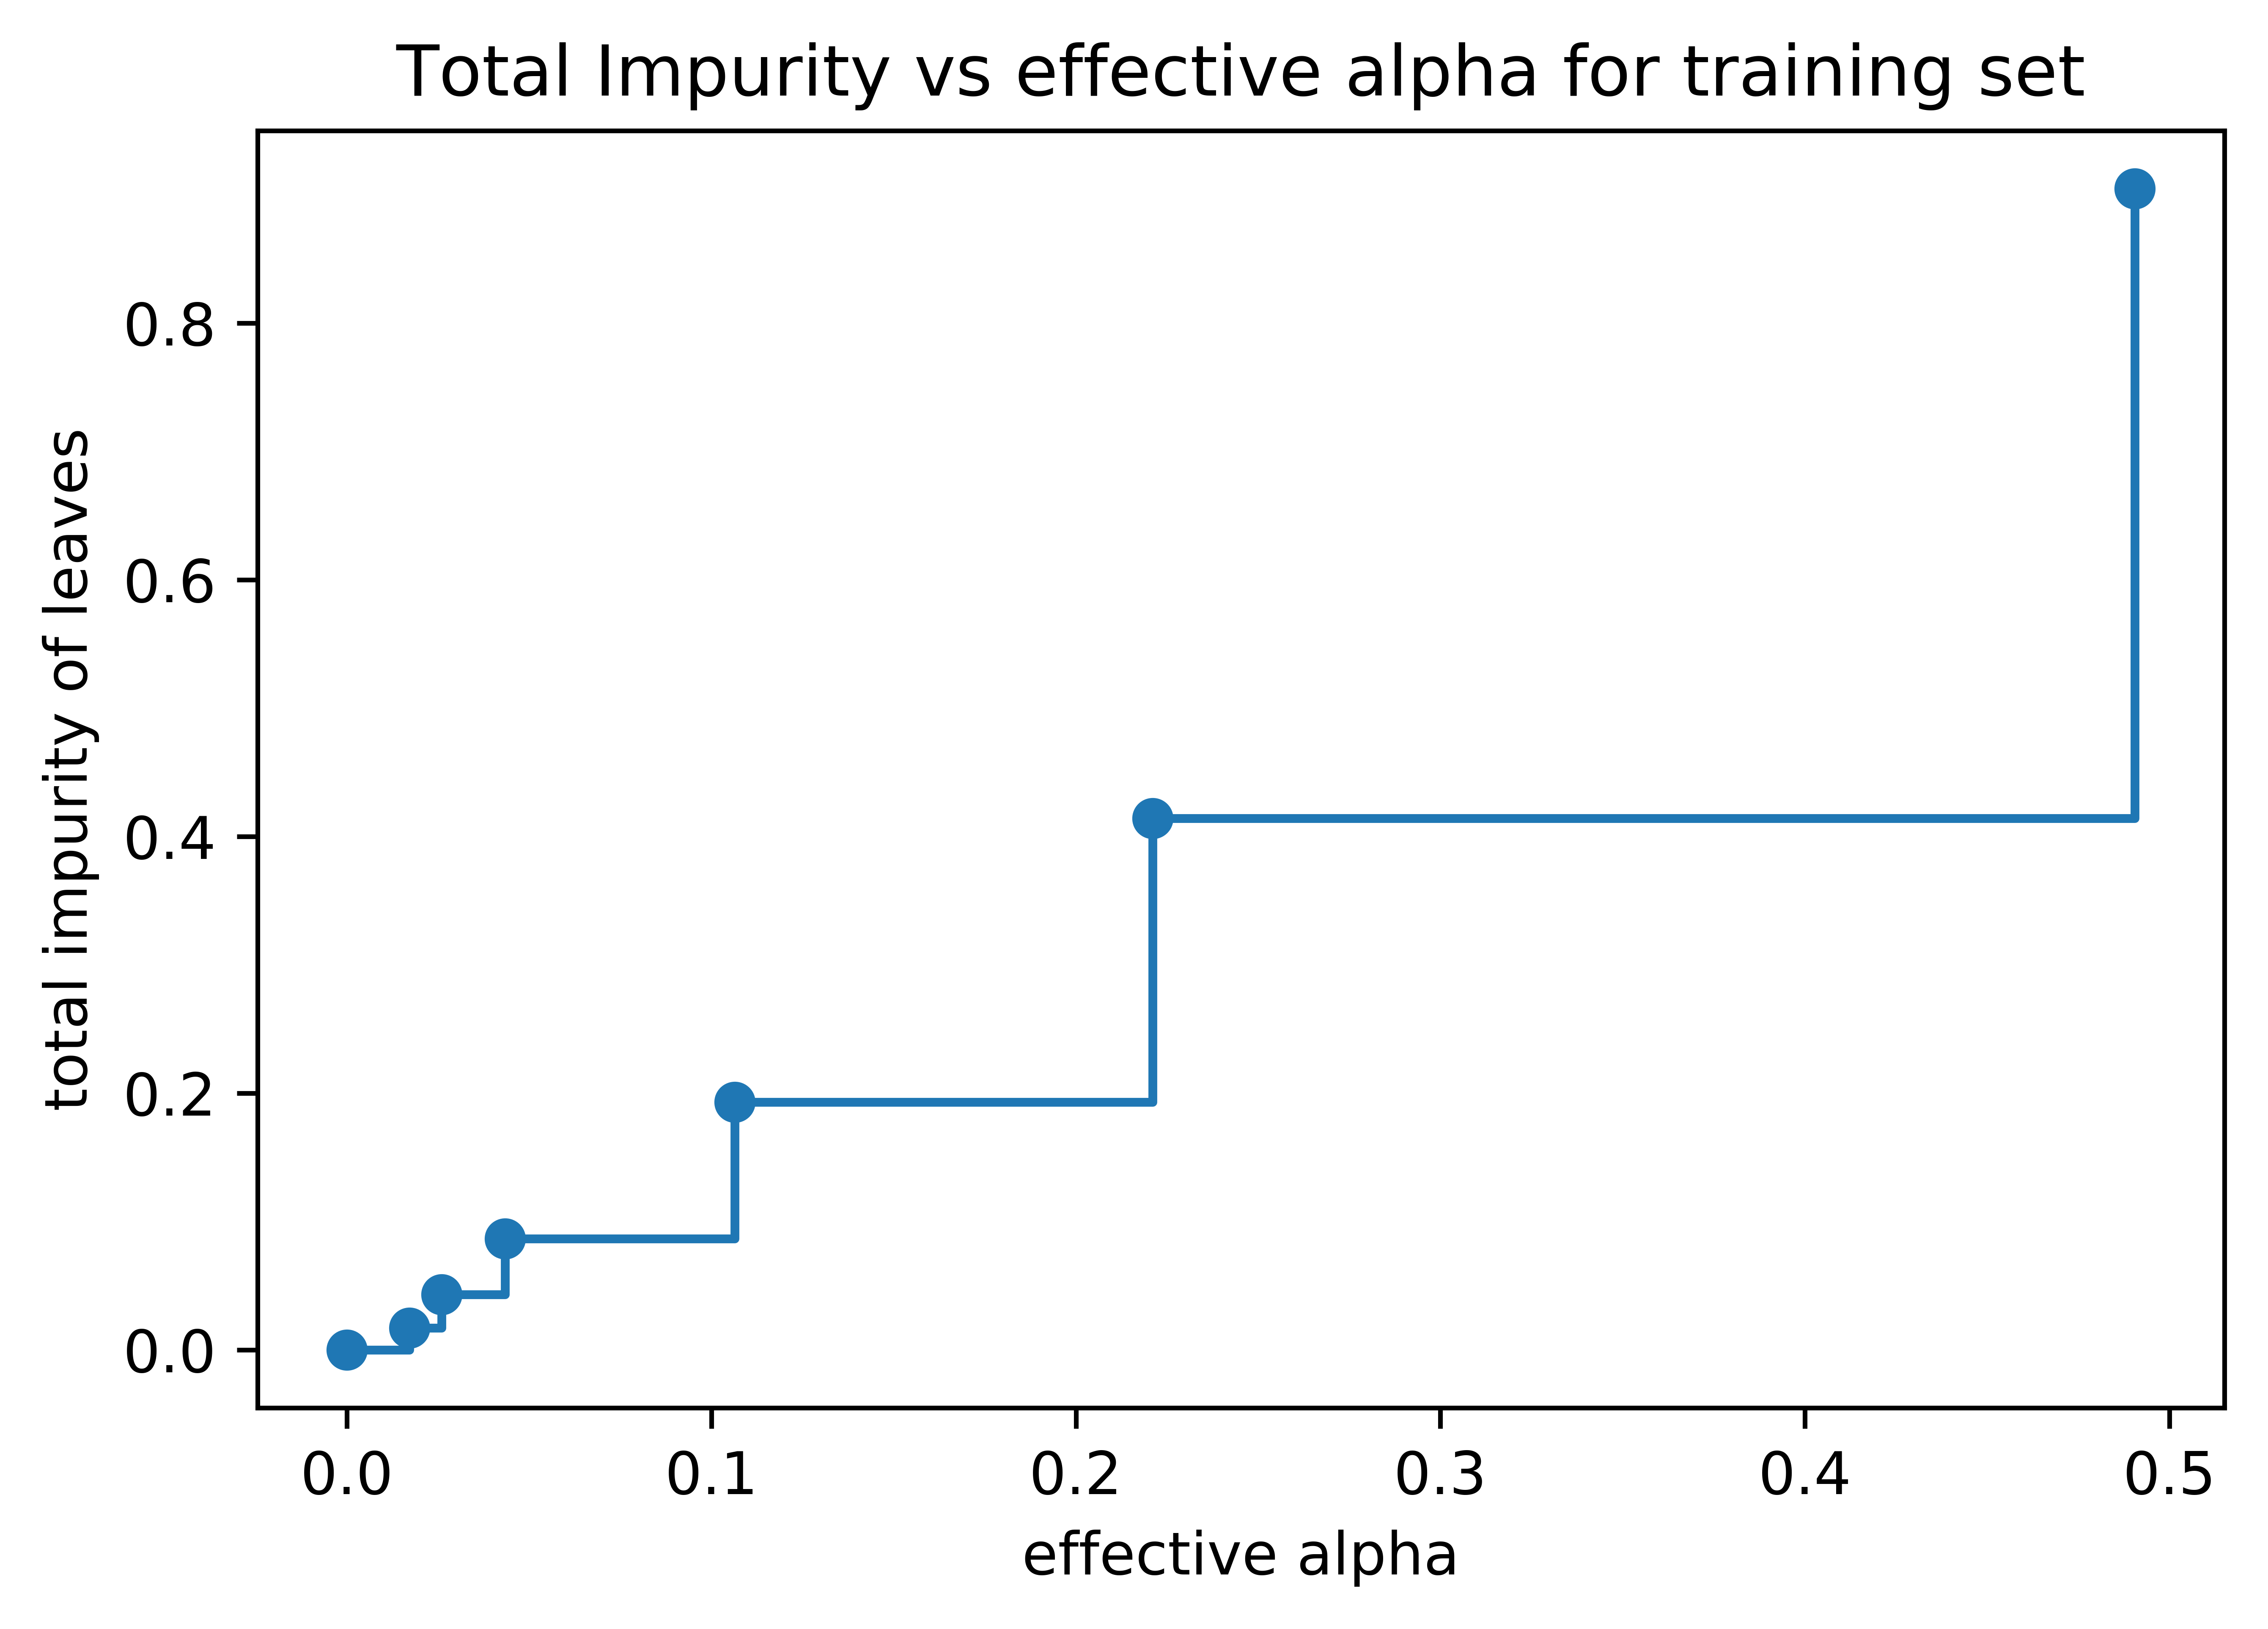
\includegraphics[width=0.7\textwidth]{1.png}
	\bicaption{总不纯度随$\alpha$值变化关系}{Total Impurity vs $\alpha$}
\end{figure}
\par 
随后考虑结点个数和决策树深度随$\alpha$值变化的关系,如\textbf{图4}所示。
\begin{figure}[h]
	\centering
	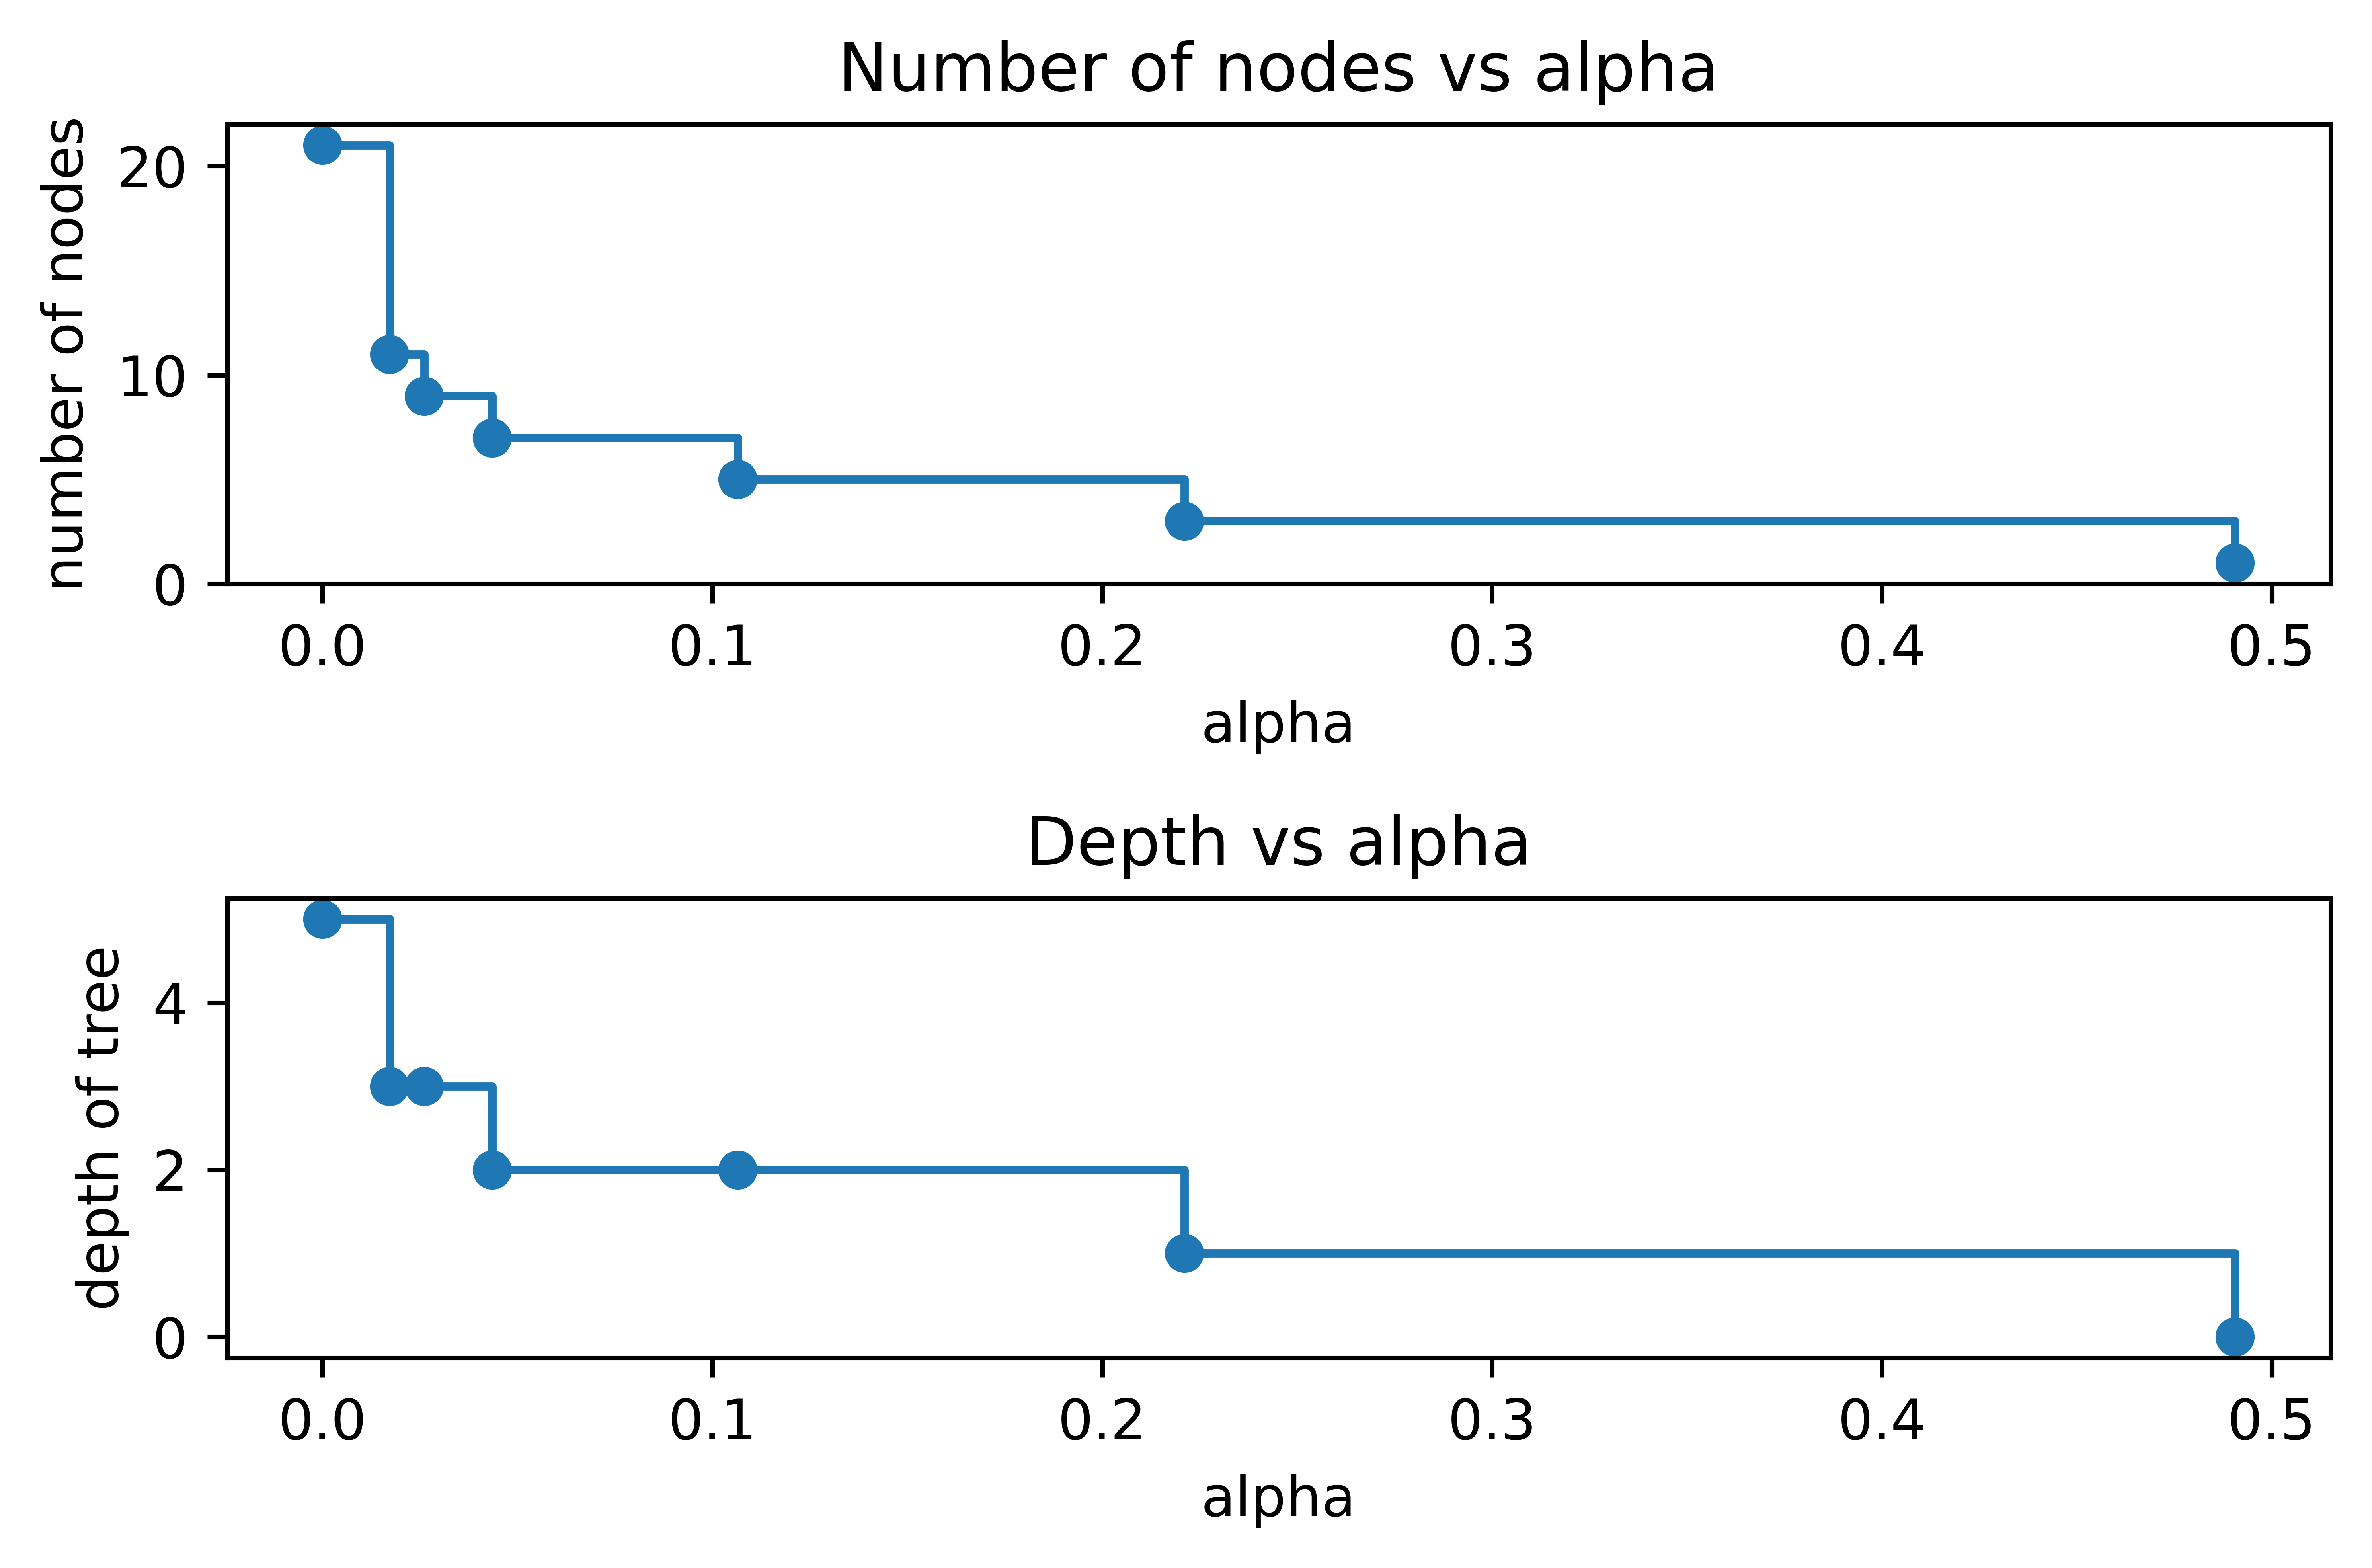
\includegraphics[width=0.7\textwidth]{2.png}
	\bicaption{结点个数和决策树深度随$\alpha$值变化关系}{Number of Nodes and Depth vs $\alpha$}
\end{figure}
\par
根据\textbf{图3}、\textbf{图4}可以看出,随着剪枝进行,$\alpha$值不断增大,而总不纯度随之不断增大,结点个数与决策树深度随之不断减小,这与前述理论分析是一致的。\par 
下面考察不同$\alpha$值对应决策树在训练集和测试集上的预测准确率,如\textbf{图5}所示。\par 
\begin{figure}[h]
	\centering
	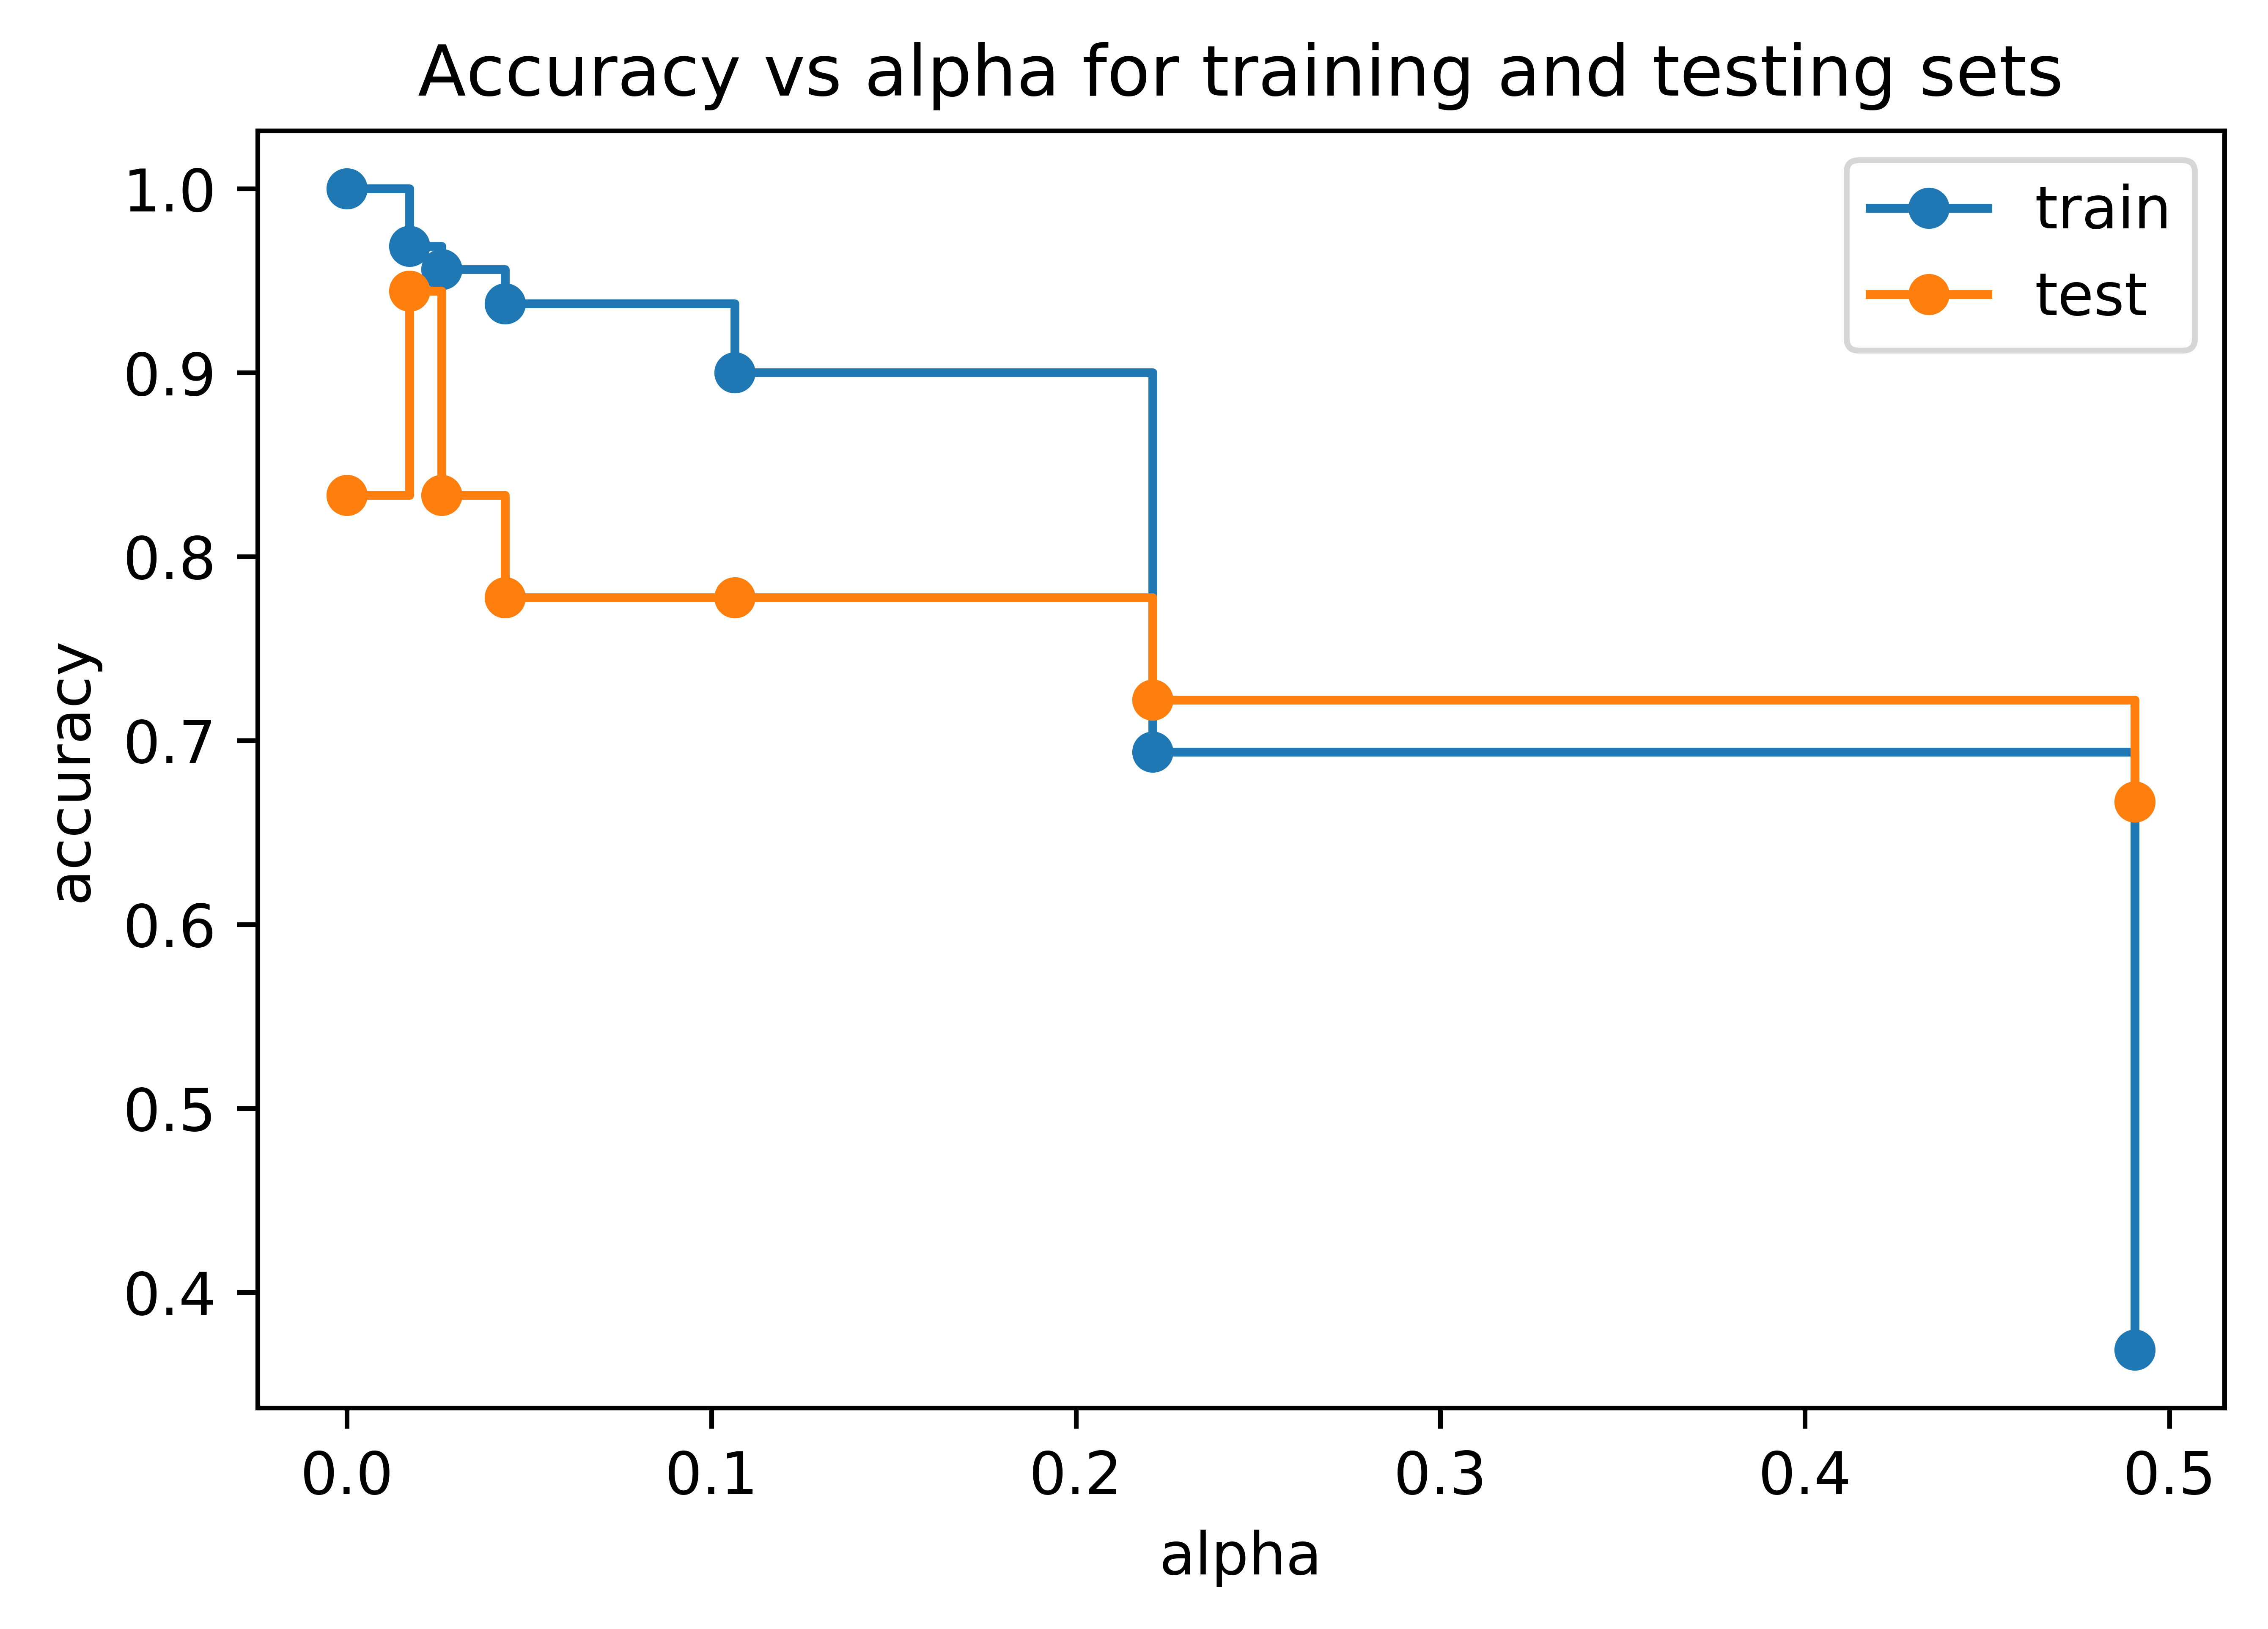
\includegraphics[width=0.7\textwidth]{3.png}
	\bicaption{训练集和测试集上准确率随$\alpha$值变化关系}{Accuracy vs $\alpha$}
\end{figure}
\par
根据\textbf{图5},可见随着剪枝的进行即$\alpha$的增大,决策树在训练集上的准确率不断降低,但在测试集上的准确率先升高再降低。这说明$\alpha$较小即决策树较深时产生了一定的过拟合现象,降低了决策树在测试集上的泛化性能。因此,CCP剪枝算法选取测试集上预测准确率最高的决策树作为剪枝后的决策树,从而一定程度上提高了决策树的泛化性能。\par 
使用CCP剪枝算法对C4.5决策树进行训练,在测试集上的平均准确率为0.9198。
\subsection{结果分析}
对比1.5和2.5的实验结果,可以分析认定:对于本题所用的wine数据集,CCP剪枝算法生成的C4.5决策树在测试集上的准确率(0.9198)略低于1.5中未剪枝的C4.5决策树(0.9342),CCP剪枝算法并未很好地实现对决策树泛化能力的提高。\par 
分析原因,考虑到\textbf{图1}所示的未剪枝的C4.5决策树深度并不太深,未出现明显的过拟合现象,并且在实际实验中所用的wine数据集样本数较少,不同的训练集/测试集划分对产生的决策树有较大影响,因此导致CCP剪枝算法未能很好提升C4.5决策树在wine数据集上的泛化性能。\par 为进一步证明上述结论,考虑到\textbf{图2}中未剪枝的CART决策树呈现出较明显的过拟合倾向,对CART决策树使用类似的CCP剪枝算法进行处理,得到的剪枝后CART决策树在测试集上的平均预测准确率为0.9237,高于未剪枝时的0.8989,证明该CCP剪枝算法具有一定的实用价值,尤其对于出现严重过拟合现象的决策树具有很好的提升泛化性能的作用。

   

\vbox{}

\bibliographystyle{ieeetr}
\bibliography{b}



\end{document}